\question[15] Escribe el grupo, subgrupo, período y clasificación de los siguientes elementos. Después de realizar este ejercicio, ubica a cada elemento en la tabla
periódica que se muestra abajo.

\begin{table}[H]
    \centering
    \begin{tabular}{c>{\columncolor[HTML]{FFCCC9}}cc>{\columncolor[HTML]{AADDFF}}cc}
                  & Grupo & Subgrupo & Período & Tipo de elemento  \\ \hline
        Polonio   &       &          &         &                   \\    \hline
        Manganeso &       &          &         &                   \\    \hline
        Magnesio  &       &          &         &                   \\    \hline
        Xenón     &       &          &         &                   \\    \hline
        Silicio   & 4     & A        & 3       & Carbonoideos      \\    \hline
        Criptón   &       &          &         &                   \\    \hline
        Fósforo   & 5     & A        & 3       & Nitrogenoides     \\    \hline
        Selenio   &       &          &         &                   \\    \hline
        Nitrógeno &       &          &         &                   \\    \hline
        Neón      & 8     & A        & 2       & Gases nobles      \\    \hline
        Bromo     &       &          &         &                   \\    \hline
        Calcio    &       &          &         &                   \\    \hline
        Oro       &       &          &         &                   \\    \hline
        Rubidio   & 1     & A        & 5       & Metales alcalinos \\    \hline
        Hidrógeno &       &          &         &                   \\    \hline
        Carbono   &       &          &         &                   \\    \hline
    \end{tabular}
\end{table}
\begin{figure}[H]
    \centering
    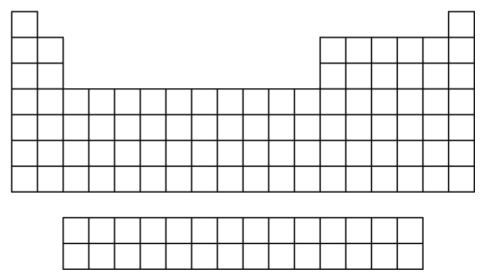
\includegraphics[width=0.9\linewidth]{../images/blank-periodictable}
\end{figure}